%%========================================================================
%% LaTeX sjabloon voor stage/projectrapport of bachelorproef
%%  HoGent Bedrijf en Organisatie
%%========================================================================

%%========================================================================
%% Preamble
%%========================================================================

\documentclass[pdftex,a4paper,12pt,twoside]{report}

% XXX: Let op: dit sjabloon is gemaakt om dubbelzijdig af te drukken
% Voor enkelzijdig, verwijder ``twoside'' hierboven.

%%---------- Extra functionaliteit ---------------------------------------

\usepackage[utf8]{inputenc}  % Accenten gebruiken in tekst (vb. é ipv \'e)
\usepackage{amsfonts}        % AMS math packages: extra wiskundige
\usepackage{amsmath}         %   symbolen (o.a. getallen-
\usepackage{amssymb}         %   verzamelingen N, R, Z, Q, etc.)
\usepackage[dutch]{babel}    % Taalinstellingen: woordsplitsingen,
                             %  commando's voor speciale karakters
                             %  ("dutch" voor NL)
\usepackage{eurosym}         % Euro-symbool €
\usepackage{geometry}
\usepackage{graphicx}        % Invoegen van tekeningen
\usepackage[pdftex,bookmarks=true]{hyperref}
                             % PDF krijgt klikbare links & verwijzingen,
                             %  inhoudstafel
\usepackage{listings}        % Broncode mooi opmaken
\usepackage{multirow}        % Tekst over verschillende cellen in tabellen
\usepackage{rotating}        % Tabellen en figuren roteren
\usepackage{natbib}          % Betere bibliografiestijlen
\usepackage{fancyhdr}        % Pagina-opmaak met hoofd- en voettekst

\usepackage[T1]{fontenc}     % Ivm lettertypes
\usepackage{lmodern}
\usepackage{textcomp}
\usepackage{listings}

\usepackage{lipsum}          % Voor vultekst (lorem ipsum)

\usepackage{float}
\usepackage{glossaries}
\makenoidxglossaries

\newglossaryentry{tracker}
{
  name=tracker,
  description={Een soort van cookie waarbij een logboek van de online activiteiten van een gebruiker worden gekoppeld aan zijn Internet Protocol(IP) adres. De tracker stuurt deze informatie door naar een externe database voor analyse. Samen met gegevens van miljoenen anderen worden die gegevens dan gebruikt voor bijvoorbeeld marketing analyse. Deze tracker blijft werken ook al heeft men de site waar de tracker gedownload werd  al lang verlaten.  },
	plural={trackers},
}
\newglossaryentry{cross-site request}
{
  name=cross-site request,
  description={Een cross-site request is een request naar een volledig andere webpagina, die de browser in opdracht van een webpagina uitvoerd. },
	plural={cross-site requests}
}
\newglossaryentry{Affiliate marketing}
{
  name=Affiliate marketing,
  description={
	Affiliate marketing is een vorm van internetmarketing waarbij adverteerders hun partners (affiliates) belonen voor de gegenereerde verkopen of leads (zoals lidmaatschappen - abonnementen) die de affiliate heeft aangeleverd. Affiliates kunnen dit bewerkstelligen door onder andere advertenties van adverteerders op hun website te plaatsen. Als er uit het doorverwijzen van klanten naar de adverteerders een verkoop of lead volgt, ontvangt de affiliate hiervoor een vergoeding van de adverteerder. },
	plural={Affiliate marketing}
}

\newglossaryentry{css selectors}
{
  name=css selector,
  description={In css worden selectors gebruikt om te selecteren welke delen moeten gebruik maken van een bepaalde stijl.},
	plural={css selectors}
}
\newglossaryentry{Whitelist}
{
  name=Whitelist,
  description={Een whitelist van een ad blocker is een lijst met webpagina's waarop de ad blocker uitgeschakeld zal zijn en waarbij advertenties wel getoond zullen worden.},
	plural={Whitelists}
}


%%---------- Layout ------------------------------------------------------

% hoofdingen, enz.
\pagestyle{fancy}
% enkel hoofdstuktitel in hoofding, geen sectietitel (vermijd overlap)
\renewcommand{\sectionmark}[1]{}

% lijn, wordt gebruikt in titelpagina
\newcommand{\HRule}{\rule{\linewidth}{0.5mm}}

% Leeg blad
\newcommand{\emptypage}{
\newpage
\thispagestyle{empty}
\mbox{}
\newpage
}

% Gebruik een schreefloos lettertype ipv het "oubollig" uitziende
% Computer Modern
\renewcommand{\familydefault}{\sfdefault}

% Commando voor invoegen Java-broncodebestanden (dank aan Niels Corneille)
% Gebruik: \codefragment{source/MijnKlasse.java}{Uitleg bij de code}
\newcommand{\codefragment}[2]{ \lstset{%
  language=java,
  breaklines=true,
  float=th,
  caption={#2},
  basicstyle=\scriptsize,
  frame=single,
  extendedchars=\true
}
\lstinputlisting{#1}}

%%---------- Documenteigenschappen ---------------------------------------
%% Vul dit aan met je eigen info:

% Je eigen naam
\newcommand{\student}{Tim Van Roosbroeck}

% De naam van je lector, begeleider, promotor
\newcommand{\promotor}{Sebastiaan Labijn}

% De naam van je co-promotor
\newcommand{\copromotor}{Joeri Van Steen}

% Indien je bachelorproef in opdracht van een bedrijf of organisatie
% geschreven is, geef je hier de naam.
\newcommand{\instelling}{---}

% De titel van het rapport/bachelorproef
\newcommand{\titel}{Adblocker en de impact op gratis content beschikbaar op het internet.}

% Datum van indienen
\newcommand{\datum}{29 mei 2016}

% Faculteit
\newcommand{\faculteit}{Faculteit Bedrijf en Organisatie}

% Soort rapport
\newcommand{\rapporttype}{Scriptie voorgedragen tot het bekomen van de graad van\\Bachelor in de toegepaste informatica}

% Academiejaar
\newcommand{\academiejaar}{2015-2016}

% Examenperiode
%  - 1e semester = 1e examenperiode
%  - 2e semester = 2e examenperiode
%  - tweede zit = 3e examenperiode
\newcommand{\examenperiode}{Tweede examenperiode}

%%========================================================================
%% Inhoud document
%%========================================================================

\begin{document}
%%---------- Front matter ------------------------------------------------
%% Het voorblad - Hier moet je in principe niets wijzigen.

\begin{titlepage}
\newgeometry{top=2cm,bottom=1.5cm,left=1.5cm,right=1.5cm}
  \begin{center}

    \begingroup
    \rmfamily
    
\includegraphics[width=2.5cm]{img/HG-beeldmerk-woordmerk}\\[.5cm]
    \faculteit\\[3cm]
    \titel
    \vfill
    \student\\[3.5cm]
    \rapporttype\\[2cm]
    Promotor:\\
    \promotor\\
    Co-promotor:\\
    \copromotor\\[2.5cm]
    Instelling: \instelling\\[.5cm]
    Academiejaar: \academiejaar\\[.5cm]
    \examenperiode
    \endgroup

  \end{center}
  \restoregeometry
\end{titlepage}


% Schutblad

\emptypage


\begin{titlepage}
  \newgeometry{top=5.35cm,bottom=1.5cm,left=1.5cm,right=1.5cm}
  \begin{center}

    \begingroup
    \rmfamily
    \faculteit\\[3cm]
    \titel
    \vfill
    \student\\[3.5cm]
    \rapporttype\\[2cm]
    Promotor:\\
    \promotor\\
    Co-promotor:\\
    \copromotor\\[2.5cm]
    Instelling: \instelling\\[.5cm]
    Academiejaar: \academiejaar\\[.5cm]
    \examenperiode
    \endgroup

  \end{center}
  \restoregeometry
\end{titlepage}


\begin{abstract}
% TODO: De "abstract" of samenvatting is een kernachtige (max 1 blz. voor een
% thesis) synthese van het document. In ons geval beschrijf je kort de
% probleemstelling en de context, de onderzoeksvragen, de aanpak en de
% resultaten.

\end{abstract}

\chapter*{Voorwoord}
\label{ch:voorwoord}

% TODO: Vergeet ook niet te bedanken wie je geholpen/gesteund/... heeft


\tableofcontents

\printnoidxglossaries
% Als je een lijst van afkortingen of termen wil toevoegen, dan hoort die
% hier thuis. Gebruik bijvoorbeeld de ``glossaries'' package.

%%---------- Kern --------------------------------------------------------

\chapter{Inleiding}
\label{ch:inleiding}

Samen met de toename in het gebruik van het internet, evolueerde ook het gebruik van dit medium voor publiciteitsdoeleinden. Tijdens de jaren ’90 deed het internet zijn intrede als reclamemedium. Naarmate meer en meer bedrijven het internet gebruiken om hun kennis, kunde en producten voor te stellen, groeit de gedachte om expliciet advertenties op de pagina’s van drukbezochte websites te plaatsen. Webvertising is een feit.
\\
Wat eerst op een schuchtere manier gebeurt, explodeert in de 21ste eeuw. Zowel via email (ook wel spam genaamd) als via webpagina’s worden internetgebruikers bestookt met allerhande reclameboodschappen. De technologie evolueert snel, alsook de manier waarop publiciteit gelinkt wordt aan het surfgedrag. Zoals steeds liggen excessen aan de basis van oppositie. Wat eerst leuk leek, wordt irritant. Opdringerige advertenties behoren tot de grootste ergernissen van internetgebruikers. Enkele banners worden vaak niet als probleem ervaren, maar sommige sites maken het erg bont. Dit verstoord evenwicht ligt wellicht aan de basis van het ontstaan van ad blocker software rond 2006.

% De inleiding moet de lezer alle nodige informatie verschaffen om het onderwerp te begrijpen zonder nog externe werken te moeten raadplegen \citep{Pollefliet2011}. Dit is een doorlopende tekst die gebaseerd is op al wat je over het onderwerp gelezen hebt (literatuuronderzoek).

% Je verwijst bij elke bewering die je doet, vakterm die je introduceert, enz. naar je bronnen. In \LaTeX{} kan dat met het commando \texttt{$\backslash${cite\{\}}} of \texttt{$\backslash${citep\{\}}}. Als argument van het commando geef je de ``sleutel'' van een ``record'' in een bibliografische databank in het Bib\TeX{}-formaat (een tekstbestand). Als je expliciet naar de auteur verwijst in de zin, gebruik je \texttt{$\backslash${}cite\{\}}.
% Soms wil je de auteur niet expliciet vernoemen, dan gebruik je \texttt{$\backslash${}citep\{\}}. Hieronder een voorbeeld van elk.

% \cite{Knuth1998} schreef een van de standaardwerken over sorteer- en zoekalgoritmen. Experten zijn het erover eens dat cloud computing een interessante opportuniteit vormen, zowel voor gebruikers als voor dienstverleners op vlak van informatietechnologie~\citep{Creeger2009}.

\section{Probleemstelling en Onderzoeksvragen}
\label{sec:onderzoeksvragen}

Het doel van het onderzoek is enerzijds inzicht te krijgen in de werking van adblockers en anderzijds het bepalen van de impact en de gevolgen op korte en lange termijn op de bedrijven die hun inkomsten halen uit reclame, en wat die bedrijven hun reactie is op ad blockers.
\begin{itemize}
	\item Wat is de impact, op dit moment en in de toekomst, van ad blockers op reclame inkomsten? 
	\item Op welke manieren omzeilen content providers momenteel ad blockers? Hoe zullen ze zich in de toekomst wapenen tegen ad blockers?
\end{itemize}

% TODO: Wees zo concreet mogelijk bij het formuleren van je
% onderzoeksvra(a)g(en). Een onderzoeksvraag is trouwens iets waar nog
% niemand op dit moment een antwoord heeft (voor zover je kan nagaan).


\chapter{Methodologie}
\label{ch:methodologie}

% TODO: Hoe ben je te werk gegaan? Verdeel je onderzoek in grote fasen, en
% licht in elke fase toe welke stappen je gevolgd hebt. Verantwoord waarom je
% op deze manier te werk gegaan bent. Je moet kunnen aantonen dat je de best
% mogelijke manier toegepast hebt om een antwoord te vinden op de
% onderzoeksvraag.
\chapter{Internet en publiciteit}
\label{ch:Internet en publiciteit}

\section{Evolutie van reclame}
\label{sec:Evolutie van reclame}
Online adverteren of online marketing, is een vorm van reclame die het internet gebruikt om zijn marketing boodschap over te brengen aan de consument. Sinds haar eerste verschijning in de vroege jaren negentig, is reclame op het internet exponentieel toegenomen in groei. Online adverteren omvat zoekrobot adverteren, sociale media reclame, scherm reclame zoals banners en mobiele reclame. Online adverteren is aanwezig in alle bedrijfstakken die zich op het internet bevinden.
\\
In 1994, in de dagen dat men moest inbellen om connectie te maken tot het internet, verscheen, op het eerste online magazine genaamd Hotwire, een schijnbaar onschuldige afbeelding. Dit statisch beeld was waarschijnlijk de eerste advertentie in zijn soort op het internet. Gebruikers die op de afbeelding klikten werden rechtstreeks doorverwezen naar site van de adverteerder. Deze banneradvertentie toonde de interactiviteit van het internet waar traditionele, éénrichtingsmedia zoals tv, radio en kranten te kort schoten. Adverteerders sprongen snel op de kar van online reclame en in 1999 bereikte de globale advertentie uitgaven de piek van een miljard dollar.
\begin{figure}[h!]
\centering

\includegraphics[width=12cm]{img/firstbanner}
\caption{De eerste reclame banner in 1994 op de site van het magazine Hotwire}
\label{fig: Banner-Ads}
\end{figure}
Naarmate het aantal gebruikers steeg op het internet, groeide het uit tot een goed verkoop medium. Bedrijven begonnen te investeren in e-commerce en content sites (in eerste instantie online versies van kranten en tijdschriften) en de verkoop van advertentie ruimte op deze sites. Naarmate gebruikers het internet voor meer activiteiten, zoals winkelen en entertainment gebruiken, werden de tactieken van adverteerders meer gevarieerd. Statische banners maakten plaats voor geanimeerde banners. Daarna kwamen de pop-ups en de pop-under advertenties gevolgd door de pre-roll video en misschien het belangrijkst de zoek advertentie. 
\\
Naarmate de gebruikers het internet ontdekten als brond voor informatie over producten, winkels en promoties, startte Google met de verkoop van advertentieruimte op basis van zoekopdrachten van de consument. Het Google AdWords Programma liet bedrijven toe om zichzelf aan de consument te tonen op de exacte momenten wanneer gebruikers naar hen, hun diensten of hun producten, op zoek waren. Adverteerders hadden nu de mogelijkheid om minder geld te verspillen aan consumenten die niet ontvankelijk zijn voor hun producten of diensten.
\\
Doordat zowel bedrijven als consumenten in grote getallen naar het internet kwamen voor alle vormen van entertainment en informatie vergrootte de complexiteit van het web enorm. Wat vroeger een eenvoudige samenwerking was tussen de adverteerders en de beheerders van webpagina’s begon alsmaar ingewikkelder te worden door de mogelijkheden die de adverteerders nodig hadden om dichter bij hun doelpubliek te komen. Hieruit zijn de reclame netwerken gegroeid, bedrijven die voor een deel van de opbrengst op zoek gaan naar reclame, statistieken bijhouden en die statistieken gebruiken om persoonlijkere reclame te leveren. Bedrijven die gebruik maken van zulke netwerken geven de controle van wat weergegeven wordt op hun website voor een stuk op. Wanneer het netwerk reclame van mindere kwaliteit levert of reclame levert die weinig te maken heeft met de andere inhoud van de webpagina dan kan dat de gebruikers ervaring verstoren, en dit zonder medeweten van de eigenaar van de webpagina.
\\
Een volgende stap in de evolutie om advertenties bij het juist doelpubliek te brengen was programmatic buying of programmatisch kopen. Dit is het principe van realtime bieden op advertentie ruimte om een specifieke advertentie te tonen aan een bepaalde consument en in een specifieke context. Dit wordt op grote schaal mogelijk gemaakt door allerhande algoritmes die het surfgedrag van de consument analyseren, informatie die onder meer afkomstig is van cookies en van big data.
\\
Het is mede door de exponentiële groei sinds de eerste advertenties, en soms slechte kwaliteit van reclame geleverd door de netwerken dat eerste ad blockers in 2006 het licht zagen. Daarnaast groeide het wantrouwen van de gebruiker over wat de adverteerders met hun persoonlijke informatie deden, op die nood aan privacy brachten de ad blockers ook een antwoord.

\section{Soorten reclame}
\label{sec:Soorten reclame}
\subsection{Banner en display advertising }
\label{sec Banner en display advertising }
Banners zijn reclame afbeeldingen die meestal getoond worden aan de randen van een webpagina voornamelijk aan de bovenkant en de zijkant \ref{fig: Banner-Ads}. Ze zijn vooral te vinden in nieuws websites en blogs. Ze zijn gemakkelijk te implementeren en te onderhouden. De advertenties van de banners komen meestal van reclame netwerken maar kunnen ook door eigenaars van de website beheerd en verkocht worden zoals men bij een papieren krant doet. De normale banner heeft maar een door klik percentage van 0.27\% wat laag is \cite{Chaffey2016}. Maar voor veel bedrijven zijn zaken zoals naamsbekendheid even belangrijk, bij reclame borden langs de weg of bij tv-reclame kan men namelijk ook niet doorklikken en die bestaan ook nog steeds. Door het lage doorklik percentage wordt de kostprijs van de advertentie niet bepaald aan de hand van het PPC-model maar wel aan de hand van de views. Met banners worden voornamelijk statische afbeeldingen bedoeld, wanneer er aan video of geluid fragmenten op de plaats van een banner staat spreekt men van display advertising, de overkoepelende term waar statische banners ook onder vallen.
\begin{figure}[h!]
\centering
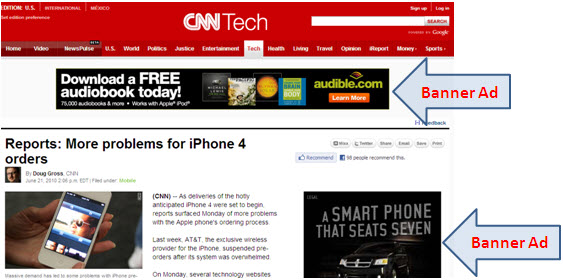
\includegraphics[width=12cm]{img/Banner-Ads}
\caption{Voorbeeld van banner ads}
\label{fig: Banner-Ads}
\end{figure}
\subsection{Google search reclame }
\label{sec Google search reclame }
Google Search reclame zijn reclame blokken die getoond worden samen met de zoek resultaten van een Google zoek opdracht, figuur:\ref{fig: Google-Search-ad}. Deze is reclame is PPC of Pay per click wat wil zeggen dat de adverteerders betalen per keer dat er op de reclame geklikt wordt. Deze reclame wordt beheerd door het Google’s AdWords platform, dat adverteerders toelaat te bieden op sleutelwoorden. Andere zoekrobotten zoals Bing en Yahoo! hebben een gelijkaardig programma.
\begin{figure}[h!]
\centering
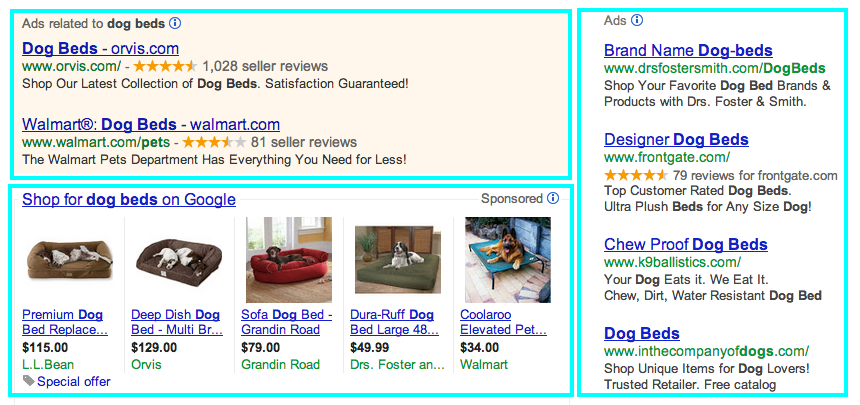
\includegraphics[width=12cm]{img/example-of-google-ads}
\caption{Voorbeeld van Google search ads}
\label{fig: Google-Search-ad}
\end{figure}
\subsection{Retargeting advertenties }
\label{sec Retargeting advertenties }
Retargeting advertenties houden rekening met de surfgeschiedenis van een gebruiker. Als een gebruiker een website bezoekt zoals Amazon of bol.com kan er een cookie gedownload worden die gebruiker volgt doorheen zijn surfsessie. Wanneer de gebruiker die site verlaat en andere websites bezoekt, zal die cookie het bezoek aan Amazon of bol.com verzenden naar reclame blokken op die andere websites. De adverteerders kunnen nu reclame maken over het product waar de gebruiker oorspronkelijk op zoek naar was op Amazon of met behulp van recommendation software gelijkaardige producten aanbieden. Deze vorm van reclame kan door gebruikers ervaren worden als een inbreuk op hun privacy.
\subsection{Sociale media advertenties }
\label{sec Sociale media advertenties }
Sociale media advertenties zijn reclame blokken op sociale netwerk diensten zoals Facebook, Twitter en Instagram. Een van de grote voordelen van deze manier van reclame maken is dat adverteerders kunnen profiteren van de grote hoeveelheid informatie die sociale media hebben over hun gebruikers. Adverteerders kunnen hun advertenties zo veel beter richten op het juiste doelpubliek.
\section{Reclame netwerken}
\label{sec:Reclame netwerken}
Een advertentienetwerk is een organisatie die als tussenpersoon dient tussen webpagina's en adverteerders. Een advertentienetwerk zal advertentieruimte van webpagina's verzamelen om deze dan te kunnen aanbieden aan adverteerders. Deze netwerken zijn er gekomen omdat het voor webpagina's moeilijk is om advertenties te verzamelen en voor adverteerders moeilijk is om advertentie ruimte te vinden voor hun doelpubliek. Naast reclame netwerken zijn er ook nog ad exchanges. Het verschil is dat men bij netwerken advertentie ruimte koopt en bij exchanges koopt men doelpubliek. Daarnaast werken exchanges via programmatisch kopen, waarbij de adverteerders in real-time bieden op het doelpubliek.


\section{Inkomsten uit reclame}
\label{sec:Inkomsten uit reclame}
Volgens het Internet Advertising Revenu verslag \cite{Silverman2015} van het Interactive Advertising Bureau, IAB, steeg de totale uitgave aan internet reclame in 2014 wereldwijd tot een historisch hoogtepunt van 135 miljard Amerikaanse dollar, met een gemiddelde groei van 17\% jaar-op-jaar.
\begin{figure}[h!]
\centering
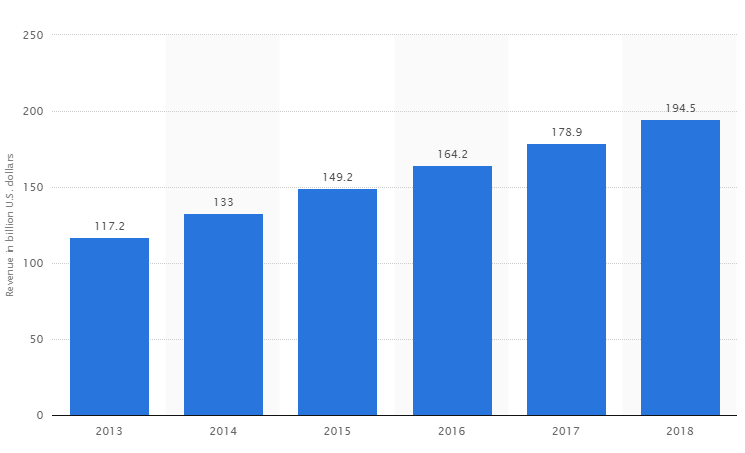
\includegraphics[width=12cm]{img/AdvertisingRevenueYearly}
\caption{Globale jaarlijkse uitgaven aan internet reclame en de voorspelling tot 2018(Miljard U.S. Dollar)}
\label{fig: AdvertisingRevenueYearly}
\end{figure} 
In zijn jaarrapport 2015 vermeldt het IAB ca 60 miljard dollar aan inkomsten uit internet advertenties in de US. In vergelijking met 2014, is dit een stijging van de omzet met ca 20\%. Deze stijging was vooral te wijten aan het succes van advertenties op mobiele toestellen, goed voor 35\% tezamen met reclame in digitale video’s (7\%). 
Met deze 60 miljard dollar reclame omzet op het internet, overstijgt het de omzet van de broadcast televisie (40 miljard) en deze van de kabel televisie (25 miljard).
De top drie omzet per industrie categorie bestaat uit: retail (22\%), financiële diensten (13\%) en auto’s (13\%). 
In zijn vooruitzichten gaat Statista \footnote{\url{www.statista.com}} uit van een substantiële stijging in 2016 van de omzet naar ca 186 miljard dollar, wereldwijd. Hiervan neemt Europa bijna 45 miljard dollar voor zijn rekening. Het aandeel van België wordt geschat op 735 miljoen dollar.

\subsection{Conclusie en vooruitzichten }
\label{Conclusie en vooruitzichten }
De analyses van verschillende studies \citep{Silverman2015,BI-Insider2016, EMarketer2016, pwc2015} bevestigen de huidige trend:

\begin{figure}[h!]
\centering
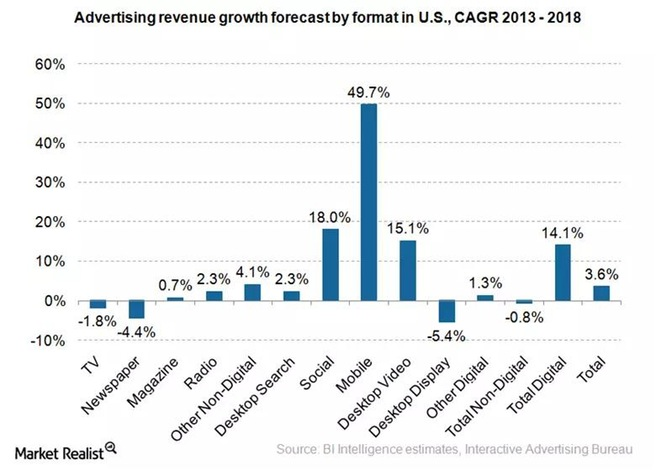
\includegraphics[width=12cm]{img/advRevGrowthFormat}
\caption{Voorspelling groei omzet onderverdeeld op media}
\label{fig: Advertising revenue growth forecast by format}
\end{figure} 

\begin{itemize}
	\item 	Tegen 2019 zal publiciteit op het internet uitgegroeid zijn tot het belangrijkste reclame medium met een vooropgestelde jaarlijkse samengestelde groei van 	12\%. Verwachte wereldomzet per 2019: 240 miljard dollar. Dit ten nadele van de meer conventionele advertentie methodieken (krant, tijdschrift, radio, televisie)
	
	\item	Deze groei zal vooral worden gerealiseerd op mobiele toestellen.
	\item	Internet advertentie technologie zal nog meer toestel bewust worden met als objectief om in alle omstandigheden dicht bij de potentiele klant te zijn (pc, tablet, smartphone, maar ook draagbare interfaces zoals uurwerken).
	\item	Betalende “Search” adverteerders zullen ongeveer 36\% van de totale omzet voor hun rekening nemen (85 miljard dollar).
	\item	Video advertentie wordt gezien als mogelijks de belangrijkste toekomstige groei factor voor de televisiezenders die op computers hun content aanbieden, vooral door de explosieve groei van de internet televisie diensten.
\end{itemize}
Bouwend op deze vooruitzichten zullen er manieren moeten gezocht worden om de inhoud van reclameboodschappen interessant te maken voor de potentiële klant afgestemd op het gebruikte toestel en zorgdragend dat dit niet lijdt tot irritaties. 

\chapter{De Ad blockers}
\label{ch:De Ad blockers}
De term ad blocker is de overkoepelende term voor alle soorten software die advertenties weg filteren of verwijderen op een webpagina. Naast het blokkeren van reclame hebben de meest gebruikte ad blockers zoals Adblock Plus en AdBlock nog andere functionaliteiten. Voorbeelden hiervan zijn het uitschakelen van tracking, en het blokkeren van Malware domeinen. Het blokkeren van advertenties zorgt er niet alleen voor dat de gebruiker een aangenamere ervaring heeft. Een ad blocker zorgt er ook voor dat webpagina’s sneller geladen worden en dat er minder bandbreedte wordt verbruikt. Doordat reclame wordt geblokkeerd zullen reclame bedrijven ook minder informatie over ad blocker gebruikers ter beschikking hebben. Met als gevolg dat de privacy beter wordt beschermd. Door het uitschakelen van trackers gaan ad blockers nog een stap verder in het beschermen van de privacy van hun gebruikers.
\section{Aanbieders}
\label{sec:Aanbieders}
\subsection{Adblock Plus}
\label{sec:Adblock Plus}
Adblock Plus\footnote{\url{https://adblockplus.org/}} is gratis extensie voor Internet Explorer, Mozilla Firefox, Google Chrome, Opera en Safari. Eyeo GmbH is het bedrijf achter Adblock Plus. Over alle browsers heen is dit de meest gebruikte ad blocker met in totaal meer dan 50 miljoen gebruikers\footnote{\url{https://chrome.google.com/webstore/search/ad\%20block?utm_source=chrome-ntp-icon&_category=extensions}} \footnote{\url{https://addons.mozilla.org/nl/firefox/extensions/?sort=users}}. Ondertussen heeft Eyeo ook haar eigen browser voor smartphones ontwikkeld waarmee nu ook advertenties op de Iphones of android toestellen geblokkeerd kunnen worden. Anders dan andere ad blockers haalt Adblock Plus zijn inkomsten niet uit donaties. Met hun "`Acceptable ads program"' laten ze bedrijven betalen om hun advertenties op een witte lijst te plaatsen.
\subsection{AdBlock}
\label{sec:AdBlock}
Adblock\footnote{\url{https://getadblock.com/}} is een gratis en opensource extensie voor Google Chrome en Safari. Het team achter AdBlock haalt zijn inkomsten volledig uit donaties. Met in totaal 40 miljoen gebruikers is dit de op één na grootste ad blocker.

\subsection{µBlock Origin}
\label{sec:uBlock Origin}
µBlock Origin\footnote{\url{https://github.com/gorhill/uBlock/}} is ook een gratis en opensource extensie voor Google Chrome en Mozilla Firefox. µBlock werkt zonder donaties en wordt door een groep vrijwilligers onderhouden en ontwikkeld. Benchmarks door µBlock zelf en \citep{PerformanceAB} tonen aan dat µBlock sneller werkt met een lagere belasting van de CPU. µBlock kan er ook voor zorgen dat scripts enkel uitgevoerd kunnen worden door vertrouwde sites. Tevens is het ook mogelijk om cross-site request te blokkeren.

\subsection{Ghostery}
\label{sec:Ghostery}
Ghostery is een gratis extensie maar niet opensource. De extensie is beschikbaar voor  Mozilla Firefox, Google Chrome, Microsoft Internet Explorer, Opera, en Safari. Ghostery Inc. is het bedrijf achter de extensie en biedt de extensie gratis aan maar verkoopt de gegevens, over de trackers en advertenties die het blokkeert, door aan derden. Ghostery focust zich voornamelijk op het beschermen van de privacy van zijn gebruikers door het blokkeren van trackers, maar verwijdert ook reclame.
\subsection{Brave}
\label{sec:Brave}
Brave is een browser die een ingebouwde ad blocker heeft en is dus geen extensie die werkt op andere browsers. De browser blokkeert niet alleen reclame en trackers maar vervangt de reclame ook met eigen advertenties. De browser is ontwikkeld door de mede oprichter van het Mozilla Project, het team achter de gelijknamige browser. Brave belooft een stuk van de inkomsten aan advertenties te delen met zowel de gebruikers als de oorspronkelijke adverteerders die hun reclame verwijderd zagen.

\section{Werking van ad blockers}
\label{ch:Werking van ad blockers}
Ad blockers zoals AdBlock en Adblock Plus hebben op zichzelf geen functionaliteit, ze moeten verteld worden wat geblokkeerd moet worden. Dit wordt mogelijk gemaakt door externe filters toe te voegen. Filters zijn in wezen een uitgebreide set van regels die een ad blocker vertellen welke elementen geblokkeerd moeten worden. De meest gebruikte filter is die van EasyList\footnote{\url{https://easylist.adblockplus.org/nl/}}. Alle eerder vernoemde ad blockers gebruiken als basis een filter van EasyList. Deze filters zijn deels regio gebonden, een Nederlandstalige filter zal een grotere focus hebben op Nederlandse (en ook Vlaamse) domeinen. Filters zijn regels tekst die bepalen welke adressen niet mogen worden geladen of welke HTML DOM Elementen niet mogen worden getoond.

\subsection{Request blocking}
\label{sec:Request blocking}
De meeste content wordt geblokkeerd door request blocking waarbij ad blockers met behulp van de filters bepalen welke HTTP of HTTPS requesten onderschept moeten worden. De filters zijn opgebouwd uit eenvoudige regels.
\\
De meest eenvoudige filter die kan gedefinieerd kan worden is bijvoorbeeld voor deze reclameblok \texttt{http://voorbeeld.com/ads/banner123.jpg}. Je kan deze regel al makkelijk beter maken door alle banners te blokkeren \texttt{voorbeeld.com/ads/banner*.jpg} of nog beter\texttt{ http://voorbeeld.com/ads/*}. Standaard zullen ad blockers voor en na elke regel een wildcard \texttt{*} zetten. De filters \texttt{advertentie}, \texttt{ad} en \texttt{*ad*} zijn dan alle drie gelijk. Het is belangrijk hier rekening mee te houden wanneer men bijvoorbeeld alle flash bestanden wil blokkeren zou men de filter \texttt{swf} kunnen toepassen. Maar deze filter zal er ook voor zorgen dat \texttt{http://voorbeeld.com/swf/index.html} zal geblokkeerd worden. De oplossing voor dit probleem is het pipe sympool |, \texttt{swf|} zal enkel adressen blokkeren die eindigen met swf. Wanneer men zowel \texttt{\textbf{http://}voorbeeld.com/banner.jpg}, \texttt{\textbf{https://}voorbeeld.com/banner.jpg} als \texttt{\textbf{https://}voorbeeld.com/banner.jpg} geblokkeerd moeten worden kan men gebruik maken van het dubbele pipe symbool: ||. \texttt{||voorbeeld.com/banner.jpg} zal de drie voorgaande adressen blokkeren.
Naast de basis regels zijn er nog meer geavanceerde regels\footnote{\url{https://adblockplus.org/en/filters}} of kan er gewerkt worden met reguliere expressies. Het gebruik van reguliere expressies wordt sterk afgeraden omdat die de performantie naar omlaag halen.
\\
Wanneer filters die in de meeste gevallen goed werken toch adressen blokkeren die niet zouden mogen geblokkeerd worden dan kunnen uitzonderingen gebruikt worden. Als de filter \texttt{adv} gebruikt wordt en \texttt{http://voorbeeld.com/advice.html} mag niet geblokkeerd worden dan kan men als uitzondering \texttt{@@advice} gebruiken. Uitzonderingsregels verschillen voor de rest niet van de filter regels en kunnen dus op dezelfde manier samengesteld worden.
\subsection{ Element hidding}
\label{sec:Element hidding}
Wanneer reclame niet kan geblokkeerd worden door request blocking, bijvoorbeeld omdat die reclame meekomt als tekst samen met de werkelijk opgevraagde webpagina, dan kan men gebruik maken van element hidding. Element hidding kan gebruikt worden als een deel van de broncode van de webpagina er bijvoorbeeld zo uit ziet:
\lstset{language=Html,tabsize=2}  
\begin{lstlisting}
	<div class="textad">
		Goedkoop bier, enkel hier en nu!
	</div>
	<div id="sponsorad">
		Goedkope pizza, klik hier!
	</div>
	<textad>
		Voor goedkoop goud, klik hier!
	</textad>
\end{lstlisting}

Men moet de webpagina downloaden, dus laadt men de reclame vanzelf ook mee. In plaats van de reclame te blokkeren kan men hier de reclame verbergen, zodat die niet zichtbaar is voor de gebruiker. Dit is waar element hidding voor bedoeld is. Element hidding regels zijn gelijkaarding opgebouwd als request blocking regels en beginnen steeds met \texttt{\#\#}. Daarnaast worden de regels opgebouwd met behulp van css selectors. In bovenstaand geval kan men bijvoorbeeld als regel \texttt{\#\#div.textad} gebruiken om de eerste reclame blok te verwijderen. Voor het tweede reclameblok en specifiek voor één domein \texttt{example.com\#\#div\#sponsorad}.

Sommige ad blockers zoals Adblock Plus en µBlock Origin beschikken over een handige tool die toelaat om manueel elementen te verbergen met behulp van een selector. Dit laat eenvoudig toe om met de muis elementen te kiezen die men liever verborgen wil zien. De ad blocker zal dan automatisch een regel genereren die bij het geselecteerde element hoort.

\section{Business model}
\label{sec:Business model}
Het business model van de instanties achter ad blockers verschilt sterk van organisatie tot ad organisatie. Er zijn ad blockers zoals µBlock Origin die volledig open source zijn en zelfs donaties weigeren. Daarnaast zijn er bedrijven zoals AdBlock die op zoek gaan naar donaties voor hun inkomsten. Anderen zoals Ghostery verzamelen, als de gebruiker hier in toestemt, informatie over de trackers en reclames op de websites die de gebruikers bezoeken. Het is belangrijk om te benadrukken dat ze geen gebruikers informatie verzamelen maar wel informatie over de bezochte website en de trackers. Die verzamelde data verkopen ze dan door aan derden.
\subsection{ Accepteable ad's program}
\label{sec:Accepteable ad's program}
Naast bovenstaande methodes is er nog een andere manier om geld te verdienen aan ad blocking, namelijk geld vragen om advertenties niet te blokkeren. Dit is het business model van Adblock Plus en is omstreden omdat hun Accepteable ad's program procedure verdacht veel lijkt op afpersing. Eén van de grote hekelpunten was dat  het systeem niet transparant genoeg werkt. Pas in december 2016 is Adblock Plus voor het eerst open geweest over hoe ze hun inkomsten vergaren. Sindsdien is op hun website een apart topic te vinden waarin uitgelegd wordt hoe ze gefinancierd worden. Een deel van de inkomsten verkijgen ze nog steeds via donaties van gebruikers.
Maar de grootste bron van inkomsten gebeurt via het Acceptable Ads program waarin ze webpagina's aan een whitelist toevoegen. De advertenties, die zich bevinden op de webpagina's die op die whitelist staan, worden niet geblokkeerd. 
Adblock Plus maakt voor whitelisting een onderscheid tussen grote en kleine advertentie eenheden. Een eenheid wordt als groot beschouwd als er een winst is van meer dan 10 miljoen extra advertentievertoningen per maand, door deelname aan het Acceptable Ads initiatief. Slechts 10\% van de whitelisting certificaten behoren tot de groep ‘grote ondernemingen’. Deze grote eenheden betalen een licentievergoeding voor het plaatsen van advertenties op de lijst. Deze vergoeding bedraagt normaal gesproken 30\% van de extra inkomsten die behaald worden door de whitelisting. 90\% van de certificaten worden echter gratis toegekend, aan kleinere advertentie eenheden. Het betalen van een licentievergoeding staat volledig los van de criteria om toegelaten te worden op de Whitelist. Zolang de Acceptable Ads criteria niet voldaan zijn, is er geen sprake van whitelisting. Er is dus geen enkele mogelijkheid om voor een advertentie die niet aan de Acceptable Ads criteria voldoet, een plaatsje op de lijst te kopen. Om de transparantie naar de buitenwereld te vergroten heeft Adblock Plus besloten om alle whitelisted advertenties en deelnemende eenheden publiek te maken op het forum van Adblock Plus \footnote{\url{https://adblockplus.org/forum/viewforum.php?f=12}}
De inkomsten van de licentievergoedingen worden onder andere gebruikt voor het onderhouden van Acceptable Ads list. Er werken vrijwilligers mee via de Adblock Plus forum community, maar het grootste deel van het beheer van de lijst (contacten met adverteerders, voortdurende controle, technische ondersteuning, …) wordt gedaan  door Eyeo GmbH, het bedrijf achter Adblock Plus.


\chapter{Evolutie gebruik Ad blockers}
\label{ch:Evolutie gebruik Ad blockers}

\section{Groei}
\label{sec:Groei}
Eind 2015 werd wereldwijd de kaap van 200 miljoen maandelijks actieve ad block gebruikers overschreden \citep{PageFair2015}. Over het volledige jaar 2015 waren er bijna 3.2 miljard\footnote{\url{ http://www.internetlivestats.com/internet-users/\#trend}} actieve internet gebruikers. Dit betekent dat meer dan 6.25\% van de internet gemeenschap een ad blocker gebruikt. Verwacht wordt dat dit percentage de komende jaren enkel maar zal stijgen. Wanneer de trend van de voorbije jaren zich voortzet dan zal het aantal gebruikers van een ad blocker jaarlijks met meer dan 40\% blijven stijgen \ref{fig: adblock-growth}.
\begin{figure}[h!]
\centering
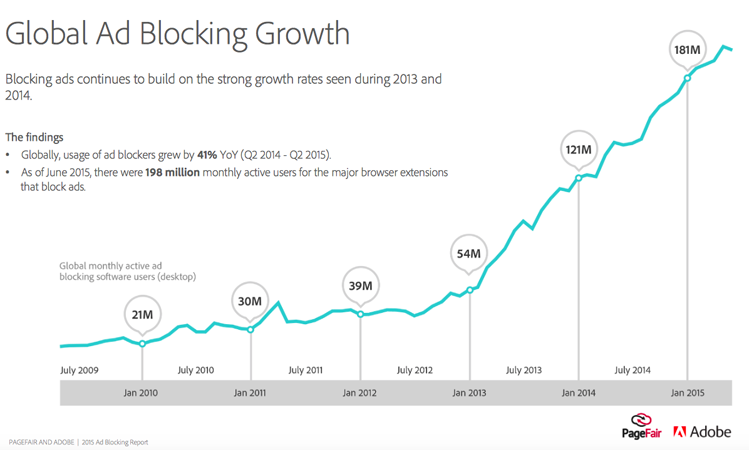
\includegraphics[width=12cm]{img/adblock-growth}
\caption{Groei van het aantal maandelijks actieve ad block gebruikers}
\label{fig: adblock-growth}
\end{figure}



\section{Spreiding}
\label{sec:Spreiding}
In 2014 en opnieuw in 2015 verzamelde PageFair samen met Adobe informatie omtrent het gebruik van ad blockers \citep{PageFair2015,PageFair2014}.

\subsection{Demografische spreiding}
\label{sec Demografische spreiding}
Ad block gebruikers zijn voor het grootste deel mannen, het is 48\% waarschijnlijker dat een man een ad blocker gebruikt bij het browsen dan een vrouw, figuur: \ref{fig: Demographic_age_sex}. Daarnaast zijn voornamelijk tieners of jonge twintigers de grootste gebruikers van ad blockers. Van de ondervraagde personen tussen de 18-29 gaf maar liefst 41\% toe een ad blocker te gebruiken. Daar komt nog eens bij dat het ook deze groep is die het meest gebruik maakt van het internet, figuur:\ref{fig: adbvsnadbHoursofIntertnet}. Het aandeel in het aantal actieve ad block gebruikers daalt met de leeftijd.

\begin{figure}[h!]
\centering
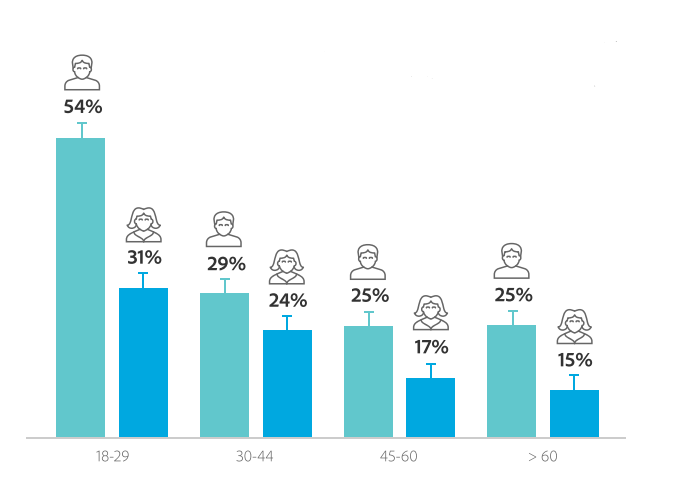
\includegraphics[width=12cm]{img/demographicsMV}
\caption{Aantal ad block gebruikers volgens leeftijd en geslacht}
\label{fig: Demographic_age_sex}
\end{figure}

\begin{figure}[h!]
\centering
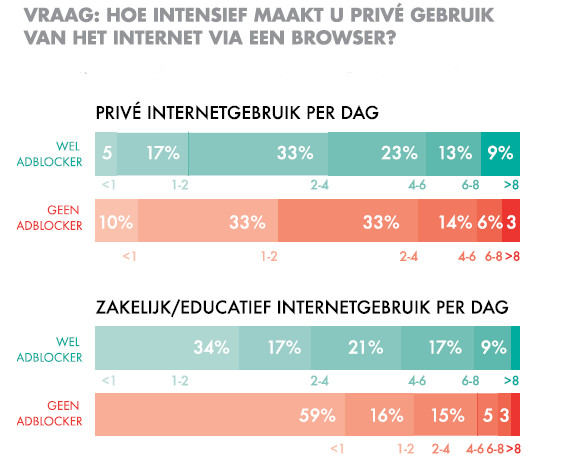
\includegraphics[width=12cm]{img/adbvsnadbHoursofIntertnet}
\caption{Gemiddeld aantal uren internet per dag: ad block gebruikers versus gebruikers zonder ad blocker, In privé en zakelijk gebruik. }
\label{fig: adbvsnadbHoursofIntertnet}
\end{figure}

\subsection{Geografische spreiding}
\label{sec Geografische spreiding}
Ad block gebruikers bevinden zich vooral in Europa en Noord-Amerika maar is nog niet doorgedrongen in Azië\footnote{\url{www.techinasia.com/adblock-plus-in-asia}}.
Griekenland en Polen zijn in Europa veruit de grootste gebruikers van ad blockers (respectievelijk 37\% en 35\%). België bengelt achteraan in de lijst met 12\%, en laat enkel Tsjechië, Frankrijk en Sovakije (8,9\%) achter zich, figuur: \ref{fig: ratespercountry}.
\begin{figure}[h!]
\centering
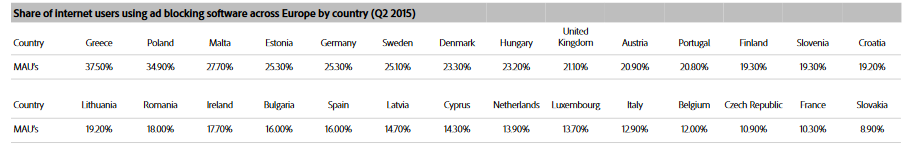
\includegraphics[width=12cm]{img/ratespercountry}
\caption{Ad block gebruik in Europa per land in procent}
\label{fig: ratespercountry}
\end{figure}

\subsection{Spreiding over de verschillende browsers en platformen}
\label{sec spreiding over de verschillende browsers}
De desktop internet browsers Chrome en Firefox hebben het grootste percentage actieve ad block gebruikers \ref{fig: Ad-blocking-by-browse}. Meer dan 35\% van de gebruikers van Firefox gebruiken een ad blocker en daarmee ligt de browser op kop. Het aantal maandelijks actieve gebruikers ligt bij Chrome wel een stuk hoger op 126 miljoen ten opzichte van de 48 miljoen van Firefox. Het gebruik van ad blockers zag bij Chrome ook een grotere toename in vergelijking met andere browsers, het gebruik steeg van 2014(Q2) naar 2015(Q2) met 51\%. Dit heeft enerzijds te maken met het gemak waarop in deze browser ad blockers kunnen gebruikt worden, maar ook met het feit dat meer en meer internet gebruikers overschakelen naar Chrome, figuur: \ref{fig: UsersPerBrowser}.
\begin{figure}[h!]
\centering
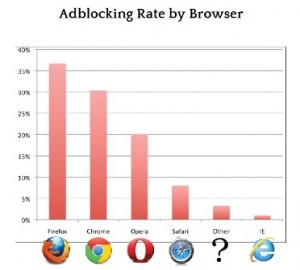
\includegraphics[width=12cm]{img/Ad-blocking-by-browse}
\caption{Percentage Ad blocker gebruikers per browser}
\label{fig: Ad-blocking-by-browse}
\end{figure}

\begin{figure}[h!]
\centering
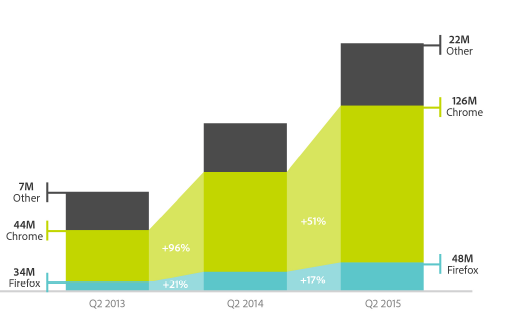
\includegraphics[width=12cm]{img/UsersPerBrowser}
\caption{Groei van het aantal maandelijkse actieve gebruikers voor Firefox en Chrome}
\label{fig: UsersPerBrowser}
\end{figure}

Er is een verschuiving zichtbaar van het percentage van internet gebruik op desktop naar dat op smartphone of tablet, figuur: \ref{fig: MobileVsDeskotpInternet}.In 2015(Q2) werd 38\% van alle web browsing op smartphone of tablet uit gevoerd. Terwijl slechts 2\% van de ad block transacties op een smartphone of tablet \cite{PageFair2015}.
Ad blocking op mobiele toestellen staat dus nog in zijn kinderschoenen.

\begin{figure}[h!]
\centering
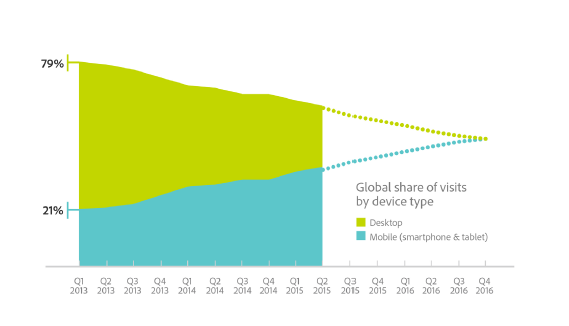
\includegraphics[width=12cm]{img/MobileVsDeskotpInternet}
\caption{Groei van het aantal maandelijkse actieve gebruikers voor Firefox en Chrome}
\label{fig: MobileVsDeskotpInternet}
\end{figure}

\subsection{Spreiding over de verschillende content}
\label{sec Spreiding over de verschillende content}
Bij webpagina's met een technisch slimmer publiek kan het gebruik van een ad blocker door de bezoekers meer de regel zijn dan de uitzondering. Gaming en social network sites hebben het hoogste ad blocking percentage: respectievelijk 26,5\% en 19,3\%, figuur:\ref{fig: percontent}. Het hoge percentage voor gaming sites ligt in lijn met het hoge percentage dat de jonge groep mannen haalt in het demografisch onderzoek. Officiële websites van overheidsinstellingen hebben het laagste percentage : 2,5\%.

\begin{figure}[h!]
\centering
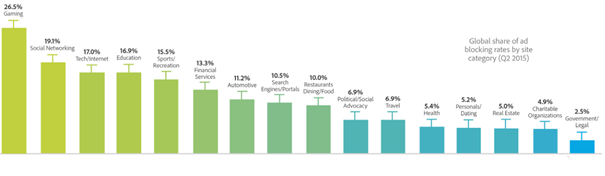
\includegraphics[width=15cm]{img/percontent}
\caption{Het aandeel van ad blockers per categorie van de webpagina, wereldwijd}
\label{fig: percontent}
\end{figure}

\subsection{Conclusie}
\label{sec Conclusie}
De gemiddelde ad block gebruiker is een man tussen de 18 en de 29 jaar en woont in Noord-Amerika of West-Europa. Dit is tevens de groep die het meest gebruik maakt van het internet. Dit zou dan ook een verklaring kunnen zijn waarom slechts 6.25\% van de internet gemeenschap een ad blocker gebruikt maar het aantal geregistreerde ad block gebruikers bij veel websites een stuk hoger ligt.%, zie hoofdstuk \ref{ch: Huidige impact van ad blockers}.

\section{Redenen voor gebruik ad blocker}
\label{sec:Redenen voor gebruik ad blocker}
Naast het blokkeren van reclame zijn er nog een aantal andere reden voor dat mensen ad blockers gebruiken. Ad blockers zorgen voor een extra laag beveiliging, ze zorgen dat webpagina's sneller worden geladen, beschermen de privacy en zorgen er ook voor dat minder bandbreedte verbruikt wordt, \cite{IAB2014}.

\begin{figure}[h!]
\centering
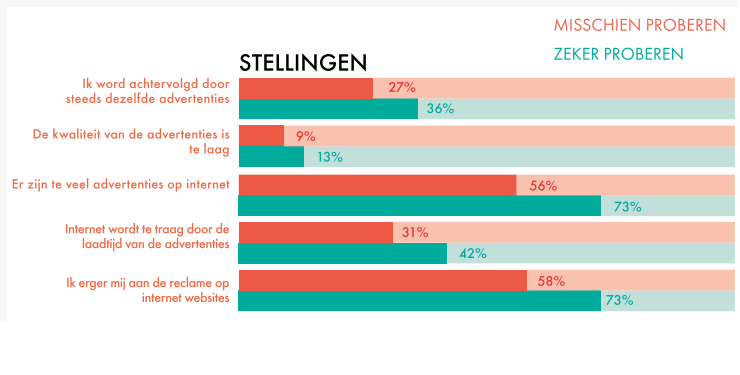
\includegraphics[width=12cm]{img/redenadblockgebruik}
\caption{Grootste ergernis van reclame op het internet in Nederland}
\label{fig: redenadblockgebruik}
\end{figure}

\subsection{Reclame}
\label{sec Reclame}
Net zoals de meeste mensen geneigd zijn om bij televisie reclame, met de afstandsbediening naar een andere zender over te schakelen, wil men bij het gebruik van internet ook de mogelijkheid hebben om advertenties te ontlopen, vooral advertenties die de ervaring van de bezoeker verstoren zijn een reden om een ad blocker installeren. De grootste ergernis vormen advertenties die niet weggeklikt kunnen worden (59\%), deze die de website grotendeels bedekken (54\%) en de advertenties met geluid (41\%), figuur: \ref{fig: Redenadblockreclame}.
\begin{figure}[h!]
\centering
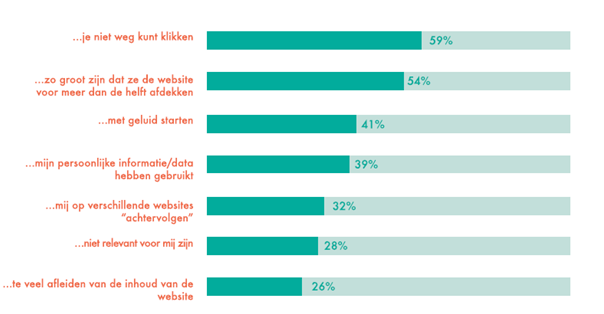
\includegraphics[width=12cm]{img/Redenadblockreclame}
\caption{Gebruikers ergeren zich het meest aan reclame die}
\label{fig: Redenadblockreclame}
\end{figure}

\subsection{Click bait}
\label{sec click bait}
Clickbait (letterlijke vertaling: ‘klikaas’) is een internetjournalistiek die inspeelt op de nieuwsgierigheid van de lezer. Ze maakt gebruik van vage, sensationele koppen in een poging om de lezer tot een klik te verleiden. De lezer wordt dan naar een site geleid vol reclame, en meestal weet het artikel de sensatie van de kop niet eens waar te maken. De site staat ook vol van andere artiekels met al even sensationele koppen, in de hoop dat de bezoeker zich opnieuw laat vangen.
\\
Voorbeelden van click bait zijn:
\begin{lstlisting}
	Mensen kunnen duizend jaar worden
	10 manieren om nooit meer moe te zijn
\end{lstlisting}


\subsection{Tracking/privacy}
\label{sec tracking/privacy}
Uit het onderzoek van Pagefair samen met Adobe, \cite{PageFair2015}, blijkt dat privacy de belangrijkste reden is voor het installeren van een ad blocker. De gebruikers willen niet dat persoonlijke informatie verzameld, geanalyseerd en gebruikt wordt door de adverteerders. Bij elke browsing sessie zijn er honderden firma's die online activiteit en browsing historiek volgen, en bijhouden. Dit is de reden dat als men eens een artikel opgezocht heeft, men blijft achtervolgd worden door advertenties in die verband houden met dit artikel. Ad blockers kunnen ingezet worden om deze tracking te vermijden. Daarvoor wordt net als voor het verwijderen van advertenties gebruik gemaakt van filterlijsten. EasyPrivacy Tracking Protection \footnote{\url{https://easylist.adblockplus.org/nl/}} List is een optioneel aanvullend abonnement, waarbij alle vormen van tracking van het internet worden verwijderd, inclusief web bugs, tracking scripts en andere informatieverzamelende elementen, waardoor je persoonlijke gegevens beschermd worden.

\subsection{Beveiliging}
\label{sec Beveiliging}
Ad blockers zijn in staat je computer te beschermen tegen malvertising. Malvertising zijn advertenties die opzettelijk bewerkt zijn met malware om de computers te besmetten van iedereen die de site waarop de advertentie staat bezoekt, ook al wordt de besmette advertentie niet eens aangeklikt. 
In de advertentie zit een stuk code dat zelfs zonder dat de advertentie geladen wordt, de computer beveiliging, van de gebruikers, onderzoekt, en dan beslist welk stuk van malware doorgestuurd wordt naar de computer. Er worden stukken software (adware) geinstalleerd op de harde schijf die je computer openstellen voor gegevensdiefstal en andere cybercriminaliteit. Als de computer door malware geïnfecteerd is, zijn de online banking gegevens, credit card informatie, wachtwoorden en andere gevoelige informatie niet meer veilig. 
Ad blockers kunnen dus gebruikt worden om zichzelf te beschermen tegen malware ( Trojan horses, wormen, spy- en adware en andere virussen). Het uitschakelen van bekende malware domeinen wordt gedaan door een nieuw filter abonnement, Malware Protection, toe te voegen. Maar een ad blocker is geen echt antivirusprogramma, het is niet aan te raden speciaal ontworpen antivirussen te vervangen door een ad blocker. 

\subsection{Laadsnelheid en bandbreedte}
\label{sec Laadsnelheid en bandbreedte}
De laadsnelheid van een pagina is de tijd die nodig is om een pagina volledig te laden nadat een gebruiker de pagina heeft geopend. De bandbreedte die webpagina verbruikt, is het aantal MegaByte dat geladen wordt bij het openen van een pagina. Bandbreedte is vooral van belang wanneer de verbinding met het internet over een connectie verloopt waarbij elke verbruikte MegaByte aangerekend wordt, zoals smartphones en andere mobiele apparaten. Ook snelheid is voor mobiele apparaten van belang want hoe langer het duurt voor een webpagina om te laden, hoe sneller de batterij zal leeg lopen. Doordat ad blockers de reclame blokkeren, zal de laadsnelheid en het data verbruik naar dalen.
\\
Uit een onderzoek, \cite{Fraser2015}, blijkt dat de installatie van Adblock Plus het gebruik van bandbreedte met 25\% naar omlaag brengt. Wanneer de ad content ook videobeelden bevat, dan loopt de winst zelfs op tot 40\%.
The New York Times deed ook een onderzoek naar de impact van ad blockers op mobiele toestellen, \cite{nytimes2015}.
In dit onderzoek werden 12 belangrijke websites betrokken. De gegevens van het dataverkeer van zowel de advertenties als de reële krantenartikels werden onderzocht. Elke homepage werd 10 maal geladen, verspreid over 2 dagen, op een Iphone 6, met 4G mobiel network. En dit eens met de ad blocker geactiveerd, en eens gedeactiveerd. Een tweede test werd gedaan om de invloed op de levensduur van de batterij te testen. Een speciale App werd ontwikkeld om door tientallen populaire websites te gaan, in een eindeloze loop. Er werd dan getimed hoe lang het duurde voor de batterij volledig leeggelopen was.

\begin{figure}[h!]
\centering
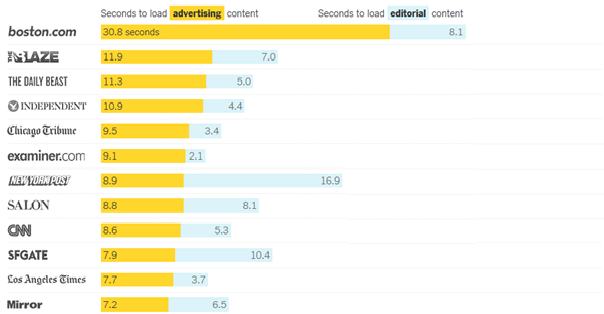
\includegraphics[width=12cm]{img/LoadTimes}
\caption{Laadtijden met en zonder ad blocker van verschillende webpagina's}
\label{fig: Redenadblockreclame}
\end{figure}

De laadtijd voor The New York Times zonder ad blocker bedraagt 7 seconden voor 3,7 MB data. Door het weglaten van de advertenties door een ad blocker , verlaagt dit tot 4 seconden voor 2,1 MB data. Het opvallendste verschil was te merken bij Boston.com. Met advertenties was er 19,4 MB data. Als de advertenties verwijderd waren door ad blocker Crystal was er 4 MB data, met 1Blocker 4,5 MB. Door het weglaten van de advertenties door een ad blocker , verlaagt de laadtijd van 39 seconden naar 8 seconden.
Ongeveer de helft van het dataverkeer komt van de advertenties, en wordt uitgefilterd bij gebruik van een ad blocker. Dit dataverkeer is ook duur. Er wordt geschat dat op een gemiddeld Amerikaanse mobiel data-abonnement, elke megabyte gedownload via een mobiele netwerk ongeveer 1 dollarcent kost . Een dagelijks bezoek aan bijvoorbeeld de home page van Boston.com, gedurende een maand zou ongeveer 9,5 dollar kosten, enkel voor het dataverkeer van de advertenties 
Uit het onderzoek valt ook op te maken dat ad blocking inschakelen op je smartphone je batterij levensduur met ongeveer 20\% verhoogt, maar deze winst geldt alleen voor de tijd dat je web browsing doet op je smartphone.
\\
Voor een aantal websites die advertenties met veel data bevat, daalt het dataverkeer aanzienlijk als ad blockers ingeschakeld zijn. De laadtijden versnellen enorm, en de levensduur van de je smarhpone batterij verhoogt ook, maar meer bescheiden.

\subsection{Conclusie}
\label{sec Conclusie}
De grootste motieven voor mensen die zeker overwegen een ad blocker te installeren zijn: irritatie over (te veel) advertenties, te trage performance en het achtervolgd worden door steeds dezelfde advertenties. Dit zijn eveneens de werkpunten waar de reclame netwerken in de toekomst best rekening mee houden. 

\chapter{Huidige impact van ad blockers}
\label{ch: Huidige impact van ad blockers}
Veel advertentiebedrijven begrijpen de redenen voor gebruik van ad blockers namelijk: snelheid, privacy, beveiliging en een webpagina zonder afleidingen. Ze beginnen te begrijpen dat voor een internet met reclame, de reclame minder agressief en storend moet worden.
\section{Impact op de internet gebruiker}
\label{sec:Impact op de internet gebruiker}
\section{Impact op de webpagina's}
\label{sec:Impact op de webpagina's}
Advertenties zorgen vaak voor een groot stuk van de inkomsten op webpagina's, sommige websites zijn zelfs volledig afhankelijk van advertenties voor hun inkomsten. De advertenties betalen voor de infrastructuur en betalen de mensen die instaan voor het onderhoud en de inhoud van een webpagina. Wereldwijd werd er in 2015 149.2 miljard dollar gespendeerd aan internet reclame. Het totale verlies aan reclame inkomsten door ad blockers bedroeg in 2015 21.88 miljard dollar \cite{PageFair2015}. Webpagina's lopen globaal gezien dus bijna 13\% van hun inkomsten mis door ad blockers. Uit interviews met verschillende content creators op YouTube en nieuws websites blijkt dat het verlies aan inkomsten oneven verdeeld is. Bij een Youtuber met de naam Driftor, die voornamelijk video's maakt die gerelateerd zijn aan videogames, loopt het verlies aan inkomsten soms op tot 45\%. Dit ligt in lijn met de onderzoeksresultaten uit hoofdstuk \ref{sec Spreiding over de verschillende content}, waaruit blijkt dat webpagina's met een grote focus op video games het grootste percentage ad block gebruikers hebben. Ook een andere Youtuber met de naam Barnacules Nerdgasm die video's maakt met een zeer technische inhoud en met onderwerpen zoals Bitcoins en 3D printing ziet meer dan 13\% van zijn inkomsten verloren gaan. Uit het interview met Barnacules blijkt dat hij 35\% van zijn doelpubliek een ad blocker gebruikt maar dat dit aantal al meer dan een jaar constant is doordat een groot stuk van zijn publiek overschakelt naar mobiele toestellen om zijn video's te bekijken. Doordat het gebruik van ad blockers op smartphones nog niet ingeburgerd is kan hij het verlies aan inkomsten door het stijgend aantal ad blockers op desktop compenseren.
Uit een interview met Peter Soetens, directeur digitale nieuwsmedia van het Mediahuis, blijkt dat ook bij hen het verlies aan inkomsten meevalt door het steeds groter aandeel van mobiele bezoekers. Mediahuis is een Belgisch mediabedrijf dat naast kranten zoals De Standaard, Het Nieuwsblad en de Gentenaar ook websites zoals Jobat heeft. Dagelijks heeft Mediahuis 1.3 miljoen digitale bezoekers waarbij op desktop 18\% van de bezoekers een ad blocker gebruikt en op mobiel minder dan 1\% een ad blocker gebruikt. Peter Soetens wist te zeggen dat het gebruik van ad blockers zeker een zorg is maar zolang het gebruik bij mobiele gebruikers laag blijft, vormen ad blockers geen echte bedreiging voor Mediahuis.


\chapter{Hoe wapenen bedrijven zich tegen ad blockers}
\label{ch:Hoe wapenen bedrijven zich tegen ad blockers}
In een poging om terug te vechten tegen het steeds groeiend gebruik van ad blockers, gebruiken websites die overleven van reclame inkomsten verschillende technieken. Van meldingen die inspelen op het geweten van de bezoekers van een webpagina, tot het volledig blokkeren van toegang voor bezoekers die een ad blocker geïnstalleerd en geactiveerd hebben.

\section{De verschillende mogelijkheden}
\label{sec:De Verschillende mogelijkheden}
Als een eigenaar of beheerder van een webpagina zijn er verschillende mogelijkheden. 

\begin{itemize}
	\item Een gebruiker kan een ad blocker detecteren en dwingen om de site niet te blokkeren of vragen een abonnement te kopen.
	\item Gebruik maken van een paywall, waarbij enkel betalende gebruikers toegang tot de content hebben.
	\item Een gelimiteerd aantal gratis bezoeken/artikels alvorens te vragen om te abonneren.
	\item Gebruikers om een vrijblijvende donatie vragen, als vervanging voor de verloren inkomsten door het gebruik van een ad blocker.
	\item Gesponsorde content
	
\end{itemize}

De keuze kan afhangen van de inhoud die de webpagina te bieden heeft, de impact die reclame heeft op de inkomstenstroom van een website, maar ook van bijvoorbeeld de loyaliteit van de bezoekers. Bij een webpagina die zich focust op verkoop van goederen of diensten zou het niet productief zijn om mensen die een ad blocker gebruiken te blokkeren, het vragen naar donaties zal ook negatief overkomen. Zelfs een melding met de vraag om de ad blocker uit te schakelen zal de gebruiker als onbeleefd ervaren.

\subsection{Blokkeren van ad block gebruikers}
\label{sec Blokkeren van ad block gebruikers}
Wanneer de verliezen van reclame inkomsten te groot worden dan kan er voor gekozen worden, om gebruikers van ad blockers toegang tot de webpagina te ontzeggen zolang de ad blocker actief is, of tot wanneer de webpagina wordt toegevoegd aan de whitelist van de ad blocker. Er kan ook aangeboden worden om een abonnement op de webpagina te kopen die het gebruik van ad blockers toe laat. Dit model wordt al toegepast door nieuwssites zoals Forbes.com en Bild.de.
\\
Het idee achter deze aanpak kan gevaarlijk zijn: in veel gevallen zien eigenaars of beheerders van webpagina's ad blocker gebruikers als niet belangrijk of niet waardevol. Ze profiteren immers van de website zonder iets in ruil te geven. Maar ze lopen zo het risico veel verkeer en de loyaliteit te verliezen, vooral bij nieuwssites waarbij het aanbod zeer uitgebreid is. Het is de loyaliteit die er voor zorgt dat gebruikers altijd opnieuw terug komen naar een specifieke webpagina en het is die loyaliteit die er in de toekomst voor kan zorgen dat gebruikers een abonnement kopen. Op lange termijn zou het dus kunnen zijn dat gebruikers blokkeren een negatief effect heeft.
\\
Wanneer men de mogelijke gevolgen op lange termijn negeert, zorgt het blokkeren van gebruikers van ad blockers voor het gewenste resultaat. Volgens een onderzoek van IAB(Internet Advertising Bureau) in het Verenigd Koninkrijk, zouden 64\% van de ondervraagden hun ad blocker uitschakelen wanneer toegang wordt geweigerd. Hieruit kan ook worden afgeleid dat 30-40\% van ad block gebruikers dit niet doen en dus wegblijven van webpagina's die hen de toegang blokkeren, en dat ze waarschijnlijk in de toekomst ook zullen wegblijven. Vooral voor webpagina's die naast hun advertenties hun inkomsten halen uit andere producten of diensten kan dit nadelig zijn.
\\
Een ander probleem zijn de beperkte technische mogelijkheden voor het detecteren en blokkeren van ad block gebruikers. Deze technieken maken gebruik van scripts die naar verloop van tijd omzeild worden door sommige ad blockers zoals µBlock. Voor sommige andere ad blockers lukt het niet om deze technieken te omzeilen, maar een extra plugin, Anti-Adblock killer, downloaden en installeren volstaat om de blokkering te omzeilen.
\\
De enige tool die er tot nu toe altijd in slaagde om elke ad blocker te detecteren is BlockAdblock \footnote{\url{http://blockadblock.com/}}.

\begin{figure}[h!]
\centering
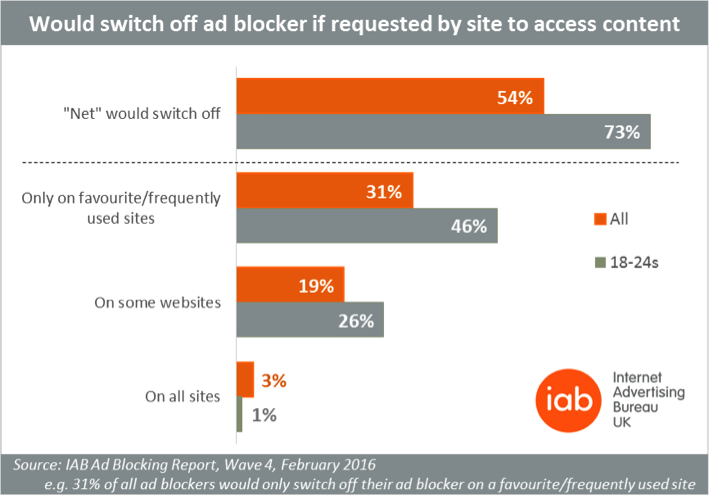
\includegraphics[width=12cm]{img/Adblockblock}
\caption{Gebruikers die beweren ad block uit schakelen wanneer toegang wordt geweigerd}
\label{fig: Adblockblock}
\end{figure}

\subsection{Gebruik maken van een paywall}
\label{sec Gebruik maken van een paywall}
Een nog hardere manier van aanpakken dan vorige methode is er voor zorgen dat niemand aan de inhoud van de betrokken webpagina kan zonder te betalen. Er wordt geen onderscheid gemaakt of de bezoeker van de webpagina een ad blocker gebruikt of niet, iedereen moet betalen. Het voordeel van deze methode is dat ze eenvoudig uit te voeren is, en dat ad blockers er niets kunnen tegen doen: er valt namelijk niets te blokkeren.
\\
Het grote nadeel is dat het bereik van je webpagina zeer klein is en zeer slecht verspreid over het internet. Gebruikers met een abonnement hebben dan wel toegang tot de content, ze kunnen er geen discussie over aangaan op sociale media want weinig kans dat vrienden en kennissen over dezelfde toegang beschikken. De Nederlandstalige nieuwssite De Correspondent \footnote{\url{https://decorrespondent.nl/}} hanteert dit model, en heeft een gedeeltelijke oplossing gevonden voor de slechte bereikbaarheid. Ze laat betalende gebruikers toe om artikels te delen op sociale media met een unieke link. Via deze link is het gedeelde artikel leesbaar voor iedereen.
\\ 
Webpagina's die dit model succesvol willen toepassen, moeten inhoud leveren van hoge kwaliteit die liefst ook uniek is. Het zal hoe dan ook moeilijk zijn om nieuwe abonnees te vinden. Een vaak gebruikte manier om toch bezoekers te lokken is om per gebruiker een aantal gratis artikels per maand ter beschikking te stellen. De gebruiker is dan wel verplicht een account aan te maken. Bezoekers kunnen via deze weg eenvoudiger verleid worden om een abonnement te kopen, ze weten beter voor welk soort content ze zullen betalen.


\subsection{Donaties vragen}
\label{sec Donaties vragen}
Bezoekers van webpagina's die een ad blocker gebruiken laten duidelijk weten dat ze de webpagina wel willen bezoeken maar daar niet alle negatieve effecten van reclame bij willen. Eigenaars en beheerders van een webpagina kunnen in plaats van reclame te tonen, donaties vragen. Ze kunnen er voor kiezen om aan niemand reclame te tonen en aan elke bezoeker een donatie te vragen, Wikipedia werkt op deze manier. Een andere mogelijkheid is aan elke gebruiker reclame te tonen en enkel bij gebruikers die deze reclame blokkeren om een donatie vragen.
\\
Het vragen van een donatie speelt in op het geweten van de gebruiker, maar het geweten van de meeste gebruikers is rap gesust. De bezoekers die ad blockers gebruiken en bereid zijn om een donatie te doen, doen dit één of misschien twee keer, waarna hun geweten gezuiverd is. Een vervanging voor de inkomsten stroom uit reclame kan dit dus niet genoemd worden.


\subsection{Gesponsorde content en affiliate marketing}
\label{sec Gesponsorde content en affiliate marketing}
Soms willen eigenaars en beheerders van webpagina's ad block gebruikers niet blokkeren of dwingen om te abonneren. Soms zijn donaties onvoldoende of men wil simpel weg niet bedelen. Dan kan men de manier waarop men adverteert aanpassen. Gesponsorde artikels zijn hier een voorbeeld van, hier betaalt een derde partij om content te plaatsen op jouw platform. Een andere mogelijk is om product reviews te publiceren die gesponsord worden door de eigenaar van dat product. 
\\
In video en beeldmateriaal kan dit op veel subtielere manieren gebeuren. Het dragen van gesponsorde kleren met merknamen op, zoals al vaker in de sport wereld gebeurt, is een eenvoudige manier om reclame in de content te verweven.
\\
Ook door middel van gesponsorde links naar andere webpagina's kan geprobeerd worden de verloren opbrengsten goed te maken.
\chapter{Toekomst}
\label{ch:Toekomst}
\section{Vooruitzicht in groei ad blockers}
\label{ch:Vooruitzicht in groei}
\subsection{Mobile}
\label{sec Mobile}
\section{Vooruitzicht in verlies opbrengsten van reclame}
\label{sec: Vooruitzicht in verlies opbrengsten van reclame}
\section{Aanpassingen aanbod publiciteit}
\label{sec:Aanpassingen aanbod publiciteit}
\subsection{Native ads}
\label{sec Native ads}
\subsection{Acceptabele ad's}
\label{sec Acceptabele ad's}
\section{Wetgevingen en rechtzaken rond ad blockers}
\label{sec:Wetgevingen en rechtzaken rond ad blockers}
Volgens de Europese wetgeving is het illegaal dat websites zonder toestemming scripts draaien op apparaten van gebruikers om te achterhalen of ze gebruik maken van ad blockers. 
In artikel 5.3 van de ePrivacy Directive staat dat het gebruik van elektronische communicatienetwerken om informatie bij de apparatuur van gebruikers op te halen of op te slaan, alleen toegestaan is wanneer heldere en volledige voorlichting hierover en een vraag om toestemming hiervoor heeft plaatsgevonden. 
De cookiewet is een voorbeeld hiervan. Maar ook ad blocker detectiescripts vallen hieronder. De Nederlandse wetgeving vormt een uitzondering op de Europese richtlijn. Als een script geen of nauwelijks inbreuk maakt op de privacy van bezoekers, is de notificatie- en toestemmingplicht niet van toepassing. Volgens de Autoriteit Persoonsgegevens is hier sprake van bij ad blocker detectiescripts. Nederlandse websites mogen dus wel ad blockers detecteren, hoeven gebruikers niet in te lichten over de detectie, en hoeven ook geen toestemming te vragen. 
\\
Sinds mei 2011, moet volgens deze Europese wet door de gebruiker altijd toestemming gegeven worden vooraleer een anti-ad blocker script kan draaien en je de toegang tot de pagina kan verbieden. Terwijl gewacht wordt op de toestemming van de bezoeker zou de site er kunnen voor kiezen om nog niets te tonen, maar zo worden de bezoekers die geen ad blockers gebruiken ook afgestraft. De pagina-inhoud tonen terwijl gewacht wordt op de toestemming heeft echter geen zin, want het was net hun bedoeling de pagina af te schermen. Dus wordt de vraag om toestemming te geven gewoon niet gesteld. Tot nu toe, wordt ook niet gecontroleerd of deze Europese wetgeving wordt toegepast.
\\
De Poolse privacy voorvechter Alexander Hanff (CEO at Think Privacy Inc.) heeft hierover in februari 2016 contact opgenomen met de Europese commissie. In april 2016 heeft hij een formele brief van hun ontvangen, waarin effectief wordt bevestigd dat anti-ad blocker scripts in strijd zijn met de Europese wetgeving. 
Met de ondersteuning van dit formele standpunt van de Europese Commissie, is Alexander Hanff van plan om aanklachten tegen meerdere EU-lidstaten in te dienen. Ook is hij bezig een website op te zetten waar een lijst bijgehouden wordt met alle websites en uitgevers die zich niet aan deze regelgeving houden. Gebruikers zullen de informatie op de site ook zelf kunnen aanvullen. Op die manier wil hij het indienen van de aanklachten vergemakkelijken.
In 2016 zijn de acties die Alexander Hanff onderneemt hieromtrent zeker verder te volgen.

\subsection{Rechtszaken}
\label{sec Rechtszaken}
Sinds 2014 hebben bedrijven en vooral uitgeverijen in verschillende Europese landen een rechtszaak aangespannen tegen het bedrijf Eyeo, de ontwikkelaar van de ad blocker Adblock Plus. Volgens de uitgevers is de software van Adblock Plus in strijd met de competitie- en copyrightwetgeving. Ze eisen dat Adblock Plus de advertenties op hun sites niet meer mag blokkeren, omdat dit een ontoelaatbare ingreep is in hun diensten, die worden gefinancierd door advertenties. 
De eisen werden in het verleden steeds afgewezen door de rechtbanken. 
\\
Een argument dat recent (april 2016) door een Duitse rechtbank werd gebruikt om de klacht te weerleggen was het volgende: de rechtbank wees erop dat Adblock Plus zich niet specifiek op de sites van de klagers richt, en dat gebruikers de standaardinstellingen kunnen aanpassen. De klacht van de betrokken uitgeverijen (Zeit Online en Handelsblatt) richtte zich voornamelijk op het acceptable-ads-initiatief van Adblock Plus. Hierbij kunnen sites, al dan niet tegen betaling, op de zogenaamde whitelist komen te staan als hun advertenties aan eisen voldoet die door Eyeo zijn opgesteld. De uitgeverijen noemen dit ronduit afpersingspraktijken.
Eyeo verdedigde zich met de verklaring dat 90\% van de sites die op de whitelist staan, niet betaald hebben en de rest, waaronder grote namen als Google en Microsoft, zou aanzienlijk meer inkomsten binnenhalen door de plaatsing op de witte lijst. 
Eerder dit jaar echter verklaarde een kleiner bedrijf tegen Financial Times 30\% van de opbrengst van de advertenties af te staan om op de whitelist te komen.
Ook tegen Brave, de nieuwe browser (gelanceerd in januari 2016) die automatisch advertenties zal blokkeren wordt al actie ondernomen. Deze browser gaat zelfs nog een stap verder: Brave blokkeert niet enkel de advertenties, maar verkoopt de vrijgekomen advertentieruimte door. 55\% van de opbrengst van deze advertentieverkoop zou volgens hen worden gedeeld met de uitgevers van de websites, maar het verwijderen van de oorspronkelijke advertenties wordt door de uitgeverijen gezien als diefstal.
In april 2016 hebben 17 Amerikaanse uitgeverijen zich gebundeld om te overwegen samen klacht in te dienen tegen Brendan Eich, de CEO en oprichter van Brave Software. Deze uitgeverijen vertegenwoordigen 1700 Amerikaanse kranten waaronder The New York Times, The Wall Street Journal, The Washington Post …
Ze dreigen een proces aan te spannen als Brave Software effectief verder gaat met zijn plan om de advertenties van de betrokken website te vervangen door advertenties van hem zelf. Tot een offciële klacht door NAA (Newspaper Association of America) kan nog niet overgegaan worden aangezien Brave Software deze manier van werken nog niet toepast. In hun aanklacht verwijzen ze ook naar een ouder proces uit 2003: een software genaamd Gator verving ook banner advertenties met eigen advertenties, gelijkaardig aan de praktijken van Brave. Een coalitie van uitgevers, waaronder Dow Jones en The New York Times, heeft het het bedrijf achter Gator aangeklaagd. Het resultaat was dat deze functie uit de software verwijderd werd.

%% TODO: de structuur en titel van deze hoofdstukken hangen af van je
% eigen onderzoek. Elke fase in je onderzoek kan een eigen hoofdstuk krijgen. Kies telkens een gepaste titel. ``Corpus'' is *GEEN* gepaste titel

\chapter{Conclusie}
\label{ch:conclusie}

% TODO: Trek een duidelijke conclusie, in de vorm van een antwoord op de
% onderzoeksvra(a)g(en). Reflecteer kritisch over het resultaat. Zijn er
% zaken die nog niet duidelijk zijn? Heeft het ondezoek geleid tot nieuwe
% vragen die uitnodigen tot verder onderzoek?



\bibliographystyle{apa}
\bibliography{tin-bachproef}

%%---------- Back matter -------------------------------------------------

\listoffigures
\listoftables

\end{document}
